\chapter[Multiple Choice Part III]{SAT Writing Multiple Choice Part III}
\section{SAT Worksheet 1C: Warm-up}

\textit{Do the following sentence improvement questions. Next to the correct answer, write an explanation about why the answer choice is correct. Next to each of the incorrect answers, write why that answer choice is incorrect.}

\begin{enumerate}
\item Two policemen were sent to check \ul{a citizen's reporting she had heard a loud party on her street.}

\begin{enumerate}[label=(\Alph*)]
\item a citizen's reporting she had heard a loud party on her street. 
\item the report of a citizen that she had heard a loud party on her street.
\item the reporting of a citizen she had heard a loud party on her street.
\item the citizen report she had heard a loud party on her street.
\item the citizen report saying a loud party on her street.
\end{enumerate}

\bigskip
\item Several of my neighbors formed a book \ul{group, for it will encourage reading and foster interesting discussions.}
\begin{enumerate}[label=(\Alph*)]
\item group, for it will encourage reading and foster interesting discussions.
\item group, in which it will encourage reading and foster interesting discussions.
\item group to encourage reading and foster interesting discussions.
\item group, that will be for the purpose of encouraging reading and fostering interesting discussions.
\item group being able to encourage reading and foster interesting discussions.
\end{enumerate}

\bigskip
\item \underline{The less you take time to exercise}, the less our endurance becomes for physical activity.
\begin{enumerate}[label=(\Alph*)]
\item The less you take time to exercise
\item The less we take time to exercise
\item The less time taken for exercise
\item The less you take time for exercising
\item As you take less for exercise
\end{enumerate}
\end{enumerate}

\newpage

\section[Paragraph Improvement]{Paragraph Improvement Questions}
The SATs have 6 questions about Improving Paragraphs. Although Improving Paragraphs questions do not make up a huge portion of the test, they are still important to your ability to do well on the Writing section and your overall score.  

\bigskip
Improving Paragraphs questions are more “big picture”: they won't ask about grammar errors within sentences, but they may ask you to improve a sentence that is too wordy, unclear, out of order, or lacking a transitional word or phrase.

\bigskip
You can think of the skills tested by the Writing Section like a series of building blocks that start small and grow bigger (though the questions don't come in this order). 

\begin{center}
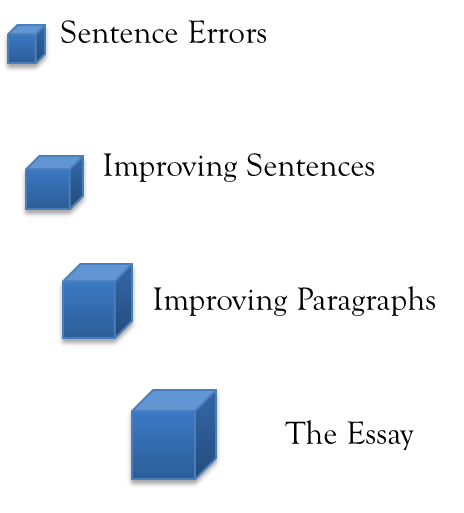
\includegraphics{Essay}
 
\end{center}

\begin{itemize}
\item{First, you have to be able to identify errors in grammar and diction. }
\item{Then, you look at sentences and figure out how to improve them.}  
\item{Improving Paragraphs questions take it to the next level—you read entire paragraphs and improve their style, organization, word choice, and clarity.}
\item{All of these skills-grammar, sentence clarity, organization-combine when you write your essay. }
\end{itemize}

\textbf{Here are the directions for Improving Paragraphs:}
\begin{center}
\textit{The following passage is an early draft of an essay. Some parts of the passage need to be rewritten.
Read the passage and select the best answers for the questions that follow. Some questions are about particular sentences or parts of sentences and ask you to improve sentence structure or word choice. Other questions ask you to consider organization and development. In making your decisions, follow the conventions of standard written English. In choosing answers, follow the requirements of standard written English.}
\end{center}

\bigskip
In other words, you will see the rough draft of an essay, 2-3 paragraphs (about 15 sentences) long.  Some questions will ask you to fix individual sentences; other questions will address the whole essay.


\bigskip   %skips added around these 2 lists so that are spread out and look better

\bigskip
\textbf{Improving Paragraphs asks you to think ``big picture"}
\begin{itemize}
\item{Clarity}
\item{Transitions between sentences, paragraphs, and ideas}
\item{Organization}
\item{Logical flow of ideas}
\end{itemize}

\bigskip

\bigskip
\textbf{Types of Questions}
\begin{enumerate}
\item{Sentence Revision - change or improve a sentence.}
\item{Sentence Addition - add a sentence or phrase to improve a transition or clarify meaning.}
\item{Sentence Combination - combine sentences using conjunctions or punctuation (e.g., a semi-colon)}
\item{Essay Analysis - identify main idea of an essay (they may ask you to give the essay a title) or improve its overall structure and mechanics.}
\end{enumerate}

\bigskip
\subsection{Strategy for Paragraph improvements}
\begin{enumerate}
\item{Quickly read over the paragraphs and take note of the \longline any grammatical errors that you see right away because there will probably be a question about that.}
\item{Then look at the \longline}
\item{Reread the sentence in context. Read the sentence \longline and the sentence \longline the line in the question}
\item{If it is a sentence improvement question, look for the “alerts” and other errors in the Writing Multiple Choice Part I and Part II.}

\bigskip
If it is a sentence addition or move question, ask yourself, “does it fit where it is, or would it be better somewhere else?” Remember: The sentences need to be coherent. Frequently, the SAT tests this by making the first part of the sentence similar to the last part of the previous sentence (that is, discussing the same topic as the second half of the previous sentence). If it doesn't discuss the topic(s) presented in the sentences around it or otherwise seems random, it may need to be removed completely. 

\bigskip
If you think that it should stay where it is, you can re-visit the option of fixing it.  If it's a run-on, try shortening it or splitting it into two sentences.  This tests the same skills as Sentence Improvement questions.  Before you “improve” the sentence though, make sure it belongs where it is!  Always consider sentences in context.

\item{Think of \longline}

\item{Look at the answer choices.  \longline the one that comes closest to your answer.}
\end{enumerate}

\section[Improvement Practice]{SAT Worksheet 2C: Exercises for Improving Paragraphs}
\textbf{\textit{Exercise \#1: Correcting Fragments}}

\bigskip
\textit{Directions: The following is an edited passage from the 1922 book, “The Outline of Science.” Read the passage and underline the sentence fragments. Then, write how you would correct these fragments to make them complete sentences.}

\bigskip
\begin{center}
\textbf{Is there Life on Mars?}
\end{center}

\begin{spacing}{2}
\begin{linenumbers*}
\modulolinenumbers[5]
\indent The basis of this belief is that if, as we saw, all the globes in our solar system are masses of metal that are cooling down, the smaller will have cooled down before the larger, and will be further ahead in their development. Now Mars is very much smaller than the earth, and must have cooled at its surface millions of years before the earth did. Hence, if a story of life began on Mars at all. We cannot guess what sort of life-forms would be evolved in a different world, but we can confidently say that they would tend toward increasing intelligence; and thus we are disposed to look for highly intelligent beings on Mars.

\indent But this argument supposes that the conditions of life, namely air and water, are found on Mars, and it is disputed whether they are found there in sufficient quantity. The late Professor Percival Lowell, who made a lifelong study of Mars, there are hundreds of straight lines drawn across the surface of the planet, and he claimed that they are beds of vegetation marking the sites of great channels or pipes by means of which the "Martians" draw water from their polar ocean. Professor W. H. Pickering, another high authority, thinks that the lines are long, narrow marshes fed by moist winds from the poles. There are certainly white polar caps on Mars. They seem to melt in the spring, and the dark fringe around them grows broader.

\indent Other astronomers, however, say that they find no trace of water-vapor in the atmosphere of Mars, and they think that the polar caps may be simply thin sheets of hoar-frost or frozen gas. And they point out that, as the atmosphere of Mars is certainly scanty, and the distance from the sun is so great.

\indent If one asks why our wonderful instruments cannot settle these points, one must be reminded that Mars is never nearer than 34,000,000 miles from the earth, and only approaches to this distance once in fifteen or seventeen years. The image of Mars on the photographic negative taken in a big telescope is very small. Astronomers rely to a great extent on the eye, which is more sensitive than the photographic plate. But it is easy to have differences of opinion as to what the eye sees.

\indent In August, 1924, the planet again be well placed for observation, and we may learn more about it. Already a few of the much-disputed lines, which people wrongly call "canals," have been traced on photographs. Astronomers who are skeptical about life on Mars are often not fully aware of the extraordinary adaptability of life. There was a time when the climate of the whole earth, from pole to pole, was semi-tropical for millions of years. No animal could then endure the least cold, yet now we have plenty of Arctic plants and animals. If the cold came slowly on Mars, as we have reason to suppose, the population could be gradually adapted to it. On the whole, it is possible that there is advanced life on Mars, and it is not impossible, in spite of the very great difficulties of a code of communication, that our "elder brothers" may yet flash across space the solution of many of our problems.
\end{linenumbers*}

\textit{Adapted from The Project Gutenberg EBook of The Outline of Science, Vol. 1 (of 4), by J. Arthur Thomson.}

\end{spacing}

\bigskip
\textbf{\textit{Exercise \#2: Transitions and Conjunctions}}
\bigskip
\textit{Directions: The following passage is taken from a student's persuasive essay advocating for a politician's support of Bill 1914 mandating driver's test for elderly drivers. Read the passage and write an appropriate transition word or phrase in the blanks.}

\begin{spacing}{2}
\begin{linenumbers*}
\modulolinenumbers[5]
\indent As a recently permitted driver, I have become familiar with some of the laws that the Massachusetts State Legislature has enacted in an attempt to curb the number of accidents involving teen drivers. These admirable bills have saved the lives of the state's children and made the roads safer for all drivers and passengers, not to mention pedestrians.\longline, it is of grave concern that there is currently very little regulation of the age group with the second highest number of motor vehicle crashes, the elderly (age sixty-five and older). The passage of proposed Bill 1914 will mandate that ``the registrar shall require that all persons aged 85 or older who are seeking to renew their operator's licenses take a vision and road test before being reissued such license". \longline I am writing to urge your support for this precedent-setting bill.

\indent Those unfit to operate a vehicle are literally “accidents waiting to happen”, jeopardizing their own lives and endangering public safety when they operate an automobile. According to the Governor's Highway Safety Bureau, older drivers were involved in 18,743 crashes in Massachusetts in 2002 \longline this age group was responsible for over 12\% of all motor vehicle fatalities. The National Highway Traffic Safety Administration reports that these statistics continue to rise steadily \longline the number of traffic-related deaths in the general population decline.

\indent Opponents of this bill may argue that since few elderly people are licensed to drive, they do not pose a serious threat on the road. This is an oversimplification \longline the number of seniors driving in Massachusetts totaled more than 858,000 in 2000. The aging of the Baby Boom generation \longline medical advancements have contributed to an increase in elderly drivers. \longline these problems can only escalate, as the National Institute on Aging predicts that in 30 years, the number of drivers over the age of eighty-five will be five times greater than today. Using this conservative estimate of the number of drivers and current accident rates, it is forecasted that this increase in population will result in the tripling of traffic fatalities caused by this age group.\longline legislation passed now will lower preventable deaths and will also have widespread implications for the future.

\indent Currently, the only people that are required to have their vision checked are first time license applicants and those persons renewing their licenses at a Registry branch. People of any age who renew their license online are exempt from this personal screening. This is relevant information \longline researchers at the University of Alabama concurred with a 1995 Johns Hopkins University study which found that state-mandated vision tests of elderly drivers are successful in lowering their accident rate.

\indent \longline Bill 1914 does not seek to deprive elders of their independence by mandating that senior citizens forfeit their license at a certain age; \hrulefill,

the bill assures that those who choose to drive are able to safely do so.
\end{linenumbers*}

\textit{Adapted from “Letter to a Representative” by Lauren Blake. Used with permission. }
\end{spacing}

\bigskip
\textbf{\textit{Exercise \#3: Sentence Order in a Paragraph}}
\bigskip
\textit{Directions: The following 5 sentences make up a paragraph about the novel The Great Gatsby. Read the sentences and then order them in the best paragraph possible. Use all 5 sentences and do not add any additional sentences. }

\bigskip
\underline{\hspace{0.5in}}He learns, however, that he can not use his power to buy the sole object of his affection, Daisy Buchannan. 

\bigskip
\underline{\hspace{0.5in}}Throughout the novel, The Great Gatsby, the character of Mr. Gatsby is at the center of this stereotype. 

\bigskip
\underline{\hspace{0.5in}}Although money correlates to economic power in 1920's American society and allows some leverage in other arenas, the powerful Mr. Gatsby is ultimately rejected by Daisy due to socio-economic class divisions.

\bigskip
\underline{\hspace{0.5in}}Images of 1920s America is one of endless parties, bootlegging, and flappers doing the Charleston all night long. 

\bigskip
\underline{\hspace{0.5in}} Coming from humble, mid-western roots and arriving at his current living situation, complete with domestic servants and a forty-acre mansion, his story seems to be the epitome of the American dream.

\bigskip
\textbf{\textit{Exercise \#4: Making an essay clearer and more concise}}
\bigskip
\textit{Directions: The following is taken from a newspaper article about paying for college. Cross out any words or phrases that you feel are redundant or should be moved in the essay.}

\begin{spacing}{2}
\begin{center}
\textbf{Show Me the Money: Getting Money For College}
\end{center}

\begin{linenumbers*}
\modulolinenumbers[5]
\indent College in the United States is extremely expensive. With tuition costing as much as \$60,000 per year, many parents and students are worried about paying for college. There are many opportunities for students to get money for school from outside organizations, government agencies, and the particular university that they hope to attend. Students can get grants or scholarships that do not have to be paid back in addition to loans, which students begin to pay back after graduation. For example, a student named Ben Kaplan was so worried about paying for Harvard that he wrote scholarship essays that earned him over \$90,000 for college.

\indent Students don't have to be the valedictorian or a star quarterback, in fact, lots of qualities, interests, and affiliations will make students eligible. Lots of different students can get money for college! Many organizations, including companies, non-profits, and unique heritage groups, award scholarships—there are scholarships for almost everything. Parents and students should start searching early in the college process and not wait until the last minute. There are national contests for high school writers, historians, and scientists, such as the Ayn Rand Essay Contests, National History Day Contest, and Intel International Science and Engineering Fair. There are many online resources such as finaid.org and fastweb.com to help students find scholarships. Students can search for books about obtaining money for college, such as How to Go to College Almost for Free, at local libraries, bookstores, and high school guidance departments.  Students can also call local businesses and associations and ask if they have any scholarships or contests with prize money.  Some national groups have awards as well.

\indent In order to get federally backed loans from their university, students need to fill out the Free Application for Federal Student Aid (FASFA) online. Each college also gives out a certain number of merit-based scholarships to attract students to their schools. After filling out the FASFA, students are sent the Student Aid Report (SAR).  Colleges use the SAT to determine student's financial aid package, that is to say colleges use this to estimate how much money a student's family can contribute to tuition and how much money a student is able to borrow. The best way to get this type of scholarship is to have a high GPA and SAT score relative to the current freshman class. Strong students are awarded merit-based scholarships. Students can also ask about the number and amount of merit-based scholarships that by calling the school or asking an admissions officer during their college visit. With scholarships and financial aid, it 'pays' to plan!
\end{linenumbers*}
\end{spacing}

\textit{Adapted from “Show Me the Money: Getting Money For College” ASC English Press Release Written April 12, 2014. Used with permission.} 


\bigskip
\textbf\textit{Exercise \#5:Dividing an Essay into Paragraphs}
\bigskip
\textit{Directions:The following is taken from student's essay contrasting the works of Robert Frost and Thylias Moss. Read the passage and decide where the sentences should be divided to in order to create four distinct paragraphs. }

\begin{spacing}{2}
\begin{linenumbers*}
\modulolinenumbers[5]
\indent The poetry of Robert Frost and Thylias Moss were influenced by different events, which attributed to the contrasting attitudes toward similar subjects in their poetry.  Frost, living in New England, was influenced by serenity and breathtaking scenes of nature. His poem, “Stopping By Woods on a Snowy Evening” epitomizes this, as the Speaker desperately desires to watch the woods fill up with snow, but regretfully acknowledges that he must continue on his journey before he can rest. With thoughts of the beauty of his home, Frost's mood is joyous. Not all poets, however, are as agreeable as he. When writing “Interpretation of A Poem By Frost”, Thylias Moss describes the filling up of woods with snow through the bleak perspective of a young African American girl. In both poems, diction and imagery work collaboratively to establish the two dissimilar tones of the authors. While Frost's attitude towards the metaphorical woods is cheery and appreciative, Moss's seems to be angry and frustrated. In creating the different tones of voice, Frost and Moss utilize contrasting choices of words. Frost utilizes passive diction, “easy wind and downy flake”, as well as end rhymes to create a pleasant atmosphere. The rhymes make the poem flow smoothly and the words sound gentle, pleasing to the ear. These combine to produce a lighter mood than in the poem by Moss. 

\indent The latter author employs words such as “inter”, “emptiness”, “polarity”, “edge” (synonymous for sharp), and “defiance”. The use of these harsh words verifies her feelings toward the subject as angry. The most apparent difference in diction, however, are the words chosen to describe the animal. Frost playfully calls the creature a “little horse” who shakes his harness bells when the Speaker stops to look at the woods. Moss refers to it as a “limited audience”, and believes the girl's efforts of defiance to be wasted on something so unworthy as a horse. Frost's lively description of the horse and entire scene contrasts Moss's degrading and cruel one, representative of Frost's relaxed tones and the overwhelming frustration felt by Moss. Both authors employ imagery and the connotations of words to establish the different emotions. Frost describes the environment: woods lovely, dark, and deep, and the frozen lake. In the background, the snow falls down softly, and the only noises are peaceful, that of a light wind and downy flake, and horse bells jingling merrily. After reading this, many imagine a peaceful scene, one which could easily be set during winter holidays (which also conjure feelings of great pleasure). On the other hand, Moss paints an entirely different picture of the landscape. In her poem, the girl is surrounded by an aura of emptiness- not welcome and serene like the former poem- but eerie and frightening. She views as the snow “inters the grass”, which for the readers results in many visualizing violent images of the snow relentlessly beating on the frail grass. Moss uses these morose images to establish her attitude towards the poem, while Frost's jovial illustrations reflect his serene attitude. The Speakers of both poems experience different metaphorical journeys, and the tones of the authors on current issues in the poems significantly affect their views of the future. The work “Stopping By Woods on a Snowy Evening” ends with the lines, “I have miles to go before I sleep, I have miles to go before I sleep”. This suggests the Speaker still has things to accomplish in his life; yet, impacted by Frost's appreciative and joyous temperament, he believes the rest of the journey- the future- will also be something to be enjoyed, as beautiful as the woods described in the beginning of the piece. While Frost's feelings of the present-day imply the future will be pleasurable, Moss's frustration continues. Moss reflects on society, believing there are, “miles to go, more than the distance from Africa to Andover, more than the distance from black to white before she sleeps with Jim”. Moss's anger stemming from prejudice influences her to predict a bleak future; she believes that racism will still be a problem, as she has observed that diverse peoples seem unwilling to cooperate and tolerate each other. The overall meaning of “Stopping By Woods on a Snowy Evening”, authored by an optimistic Robert Frost, is one should appreciate life- now and in the future; however, Thylias Moss's contrasting tone of anger and frustration expresses the challenges of a young African American, and implies unless drastic social measures are taken, intolerance will only continue.     
\end{linenumbers*}
\end{spacing}

\bigskip
\textit{Adapted from ``Comparisons Essay'' by Lauren Blake. Used with permission.}

\vfill
\newpage
\section[Improvement Practice]{SAT Worksheet 3C: Paragraph Improvements Practice Questions}

\bigskip
\textit{Directions: Read the passage and select the best answers for the questions that follow. Some questions are about particular sentences or parts of sentences and ask you to improve sentence structure or word choice. Other questions ask you to consider organization and development. In making your decisions, follow the conventions of standard written English. In choosing answers, follow the requirements of standard written English.}

\bigskip
\indent (1) Privacy is something that is guaranteed to everyone by the Constitution. (2) When you think of the right to privacy, we usually think of being comfortable at home, away from the prying eyes of others. (3) In this age of technology, we might also think of the security of personal information we put on the internet or the credit card information we give to make purchases. (4) Issues of privacy pervade more areas of our lives than we might initially imagine. (5) An example of this is the privacy policies of hospitals.

\indent (6) Hospitals are liable anytime patient privacy is violated. (7) Hospitals protect patient information as much as possible. (8) Any papers containing sensitive information are shredded and disposed of carefully when necessary. (9) Employees are expected to honor patient confidentiality and are not allowed to talk about their patients outside the hospital. (10) In the same way, lawyers uphold the same standards of privacy with their clients. (11) If patient privacy is disregarded, the consequences can be severe. (12) Big fines must be paid and dismissal from one's post is highly probable. (13) Because most employees cannot afford to face these consequences, they take great care not to violate the hospital's privacy policies.

\begin{enumerate}
\item{What is the best way to revise the underlined portion in sentence 2 (reproduced below)?}

\ul{When you think of the right to privacy, we usually think} of being comfortable at home, away from the prying eyes of others.
\begin{enumerate}[label=(\Alph*)]
\item{When you thought of the right to privacy, we usually thought}
\item{When the right to privacy is thought of, we usually think}
\item{Thinking of the right to privacy, we usually think}
\item{When we think of the right to privacy, we usually think}
\item{When you are thinking of the right to privacy, we usually think}
\end{enumerate}

\newpage
\item{In context, which of the following phrases is best to insert at the beginning of sentence 4?}
\begin{enumerate}[label=(\Alph*)]
\item{Likewise,}
\item{Furthermore,}
\item{Still,}
\item{Nevertheless,}
\item{For instance,}
\end{enumerate}

\bigskip
\item{In context, which of the following is the best version of sentence 5 (reproduced below)?}

\bigskip
\textit{An example of this is the privacy policies of hospitals.}
\begin{enumerate}[label=(\Alph*)]
\item{(as it is now)}
\item{An example of the far-reaching influence of privacy concerns is the privacy policies of hospitals.}
\item{For example, hospitals have privacy policies.}
\item{Hospital's privacy policies are an example of this.}
\item{Regarding the effect of privacy issues, hospitals have privacy policies as an example.}
\end{enumerate}

\bigskip
\item{Of the following, which is the best way to revise and combine sentences 6 and 7?}

\bigskip
\textit{Hospitals are liable anytime patient privacy is violated. Hospitals protect patient information as much as possible.}

\begin{enumerate}[label=(\Alph*)]
\item{Because hospitals are liable anytime patient privacy is violated, they protect patient information as much as possible.}
\item{Hospitals are liable anytime patient privacy is violated, therefore, they protect patient information as much as possible.}
\item{With the liability hospitals face anytime patient privacy is violated, they protect patient information as much as possible.}
\item{Protecting patient information as much as possible, hospitals are liable anytime patient privacy is violated.}
\item{Anytime patient information is violated, hospitals are liable to protect patient information as much as possible.}
\end{enumerate}

\newpage
\item{Which of the following sentences should be omitted to improve the unity of the second paragraph?}
\begin{enumerate}[label=(\Alph*)]
\item{Sentence 9}
\item{Sentence 10}
\item{Sentence 11}
\item{Sentence 12}
\item{Sentence 13}
\end{enumerate}

\bigskip
\item{Which of the following best expresses the relationship between sentences 11 and 12?}

\begin{enumerate}[label=(\Alph*)]
\item{Sentence 12 offers a solution to a problem posed in sentence 11.}
\item{Sentence 12 puts forth evidence that contradicts the point made in sentence 11.}
\item{Sentence 12 provides a transition away from the topic discussed in sentence 11.}
\item{Sentence 12 indicates a reason for the assertion made in sentence 11.} 
\item{Sentence 12 elaborates on a hypothetical result presented in sentence 11.}
\end{enumerate}
\end{enumerate}